\documentclass[aps,prd,twocolumn,superscriptaddress,showpacs,preprintnumbers,nofootinbib,longbibliography,floatfix]{revtex4-2}
\usepackage[utf8]{inputenc}
\usepackage{amsmath,amssymb}
\usepackage{graphicx}
\PassOptionsToPackage{hyphens}{url}
\usepackage[colorlinks=true,allcolors=blue]{hyperref}
\usepackage{url}
\makeatletter
\g@addto@macro\UrlBreaks{\do\/\do\_\do\-\do\.}
\makeatother
\usepackage{booktabs}
\usepackage{seqsplit}
\newcommand{\fnl}{f_{\rm NL}}
\newcommand{\eps}{\epsilon}
\newcommand{\etal}{\textit{et~al.}}
\newcommand{\paperVersion}{v1S.0.1}
\newcommand{\paperTimestamp}{September 4, 2026}

\begin{document}

\preprint{\paperVersion}

\title{When the separate universe fails: a criterion for the squeezed bispectrum\\
in non-attractor phases}

\author{Houston Golden}
\email{houston@hubify.com}
\altaffiliation[ORCID: ]{\href{https://orcid.org/0009-0008-5616-5994}{0009-0008-5616-5994}}
\affiliation{Independent Researcher, Los Angeles, California, USA}

\date{\paperTimestamp}

\begin{abstract}
The isotropic separate universe ($\delta N$) reproduces the squeezed bispectrum of $\zeta$
in ultra-slow-roll inflation, and fails by a factor of $8/3$ in a matter-dominated
contraction. We derive the exact threading identity relating $\delta N$'s zero-shift
variable $\delta N_c$ to Maldacena's $\zeta$ and state a single criterion: the two agree iff
the $\zeta$-growth-weighted mean $\langle\eps/c_s^2\rangle_\zeta$ vanishes, otherwise
$\delta N_c=(1-\langle\eps/c_s^2\rangle_\zeta/3)\,\zeta$ plus an explicit second-order
correction. The linear result is exact for any history; the second-order result is exact at
constant $\eps$, $c_s=1$, with a closed general equation-of-state form. We validate on four
cases -- matter-dominated contraction ($O(1)$ failure), ultra-slow-roll (agreement to
$O(\eps)$), attractor slow roll (identity map), ekpyrosis (passes) -- and place the result
against the non-attractor consistency-relation literature. The criterion is a second,
independent failure mode of the separate universe beyond the known initial-data requirement,
invisible to inflationary tests because it is $O(\eps)$ there and $O(1)$ in contraction.
\end{abstract}

\maketitle

\section{Motivation}

The squeezed limit of the primordial bispectrum is governed, in single-clock inflation, by
Maldacena's consistency relation, and can equivalently be computed by the separate-universe
($\delta N$) formalism, which treats the long-wavelength mode as a local shift of the
background evolution~\cite{Maldacena2003}. In a non-attractor phase, where $\dot\zeta\neq0$
on super-Hubble scales, two independent difficulties arise. First,
Namjoo, Firouzjahi \& Sasaki showed that ultra-slow-roll (USR) inflation violates the
consistency relation, $\fnl=5/2$, and that $\delta N$ built from $N(\phi)$ alone misses
this: the growing mode is an independent initial datum, requiring $N(\phi,\pi)$ to be
correctly captured~\cite{Namjoo2013}. This initial-data requirement was extended to
$P(X)$ non-attractors by Chen, Firouzjahi, Namjoo \& Sasaki, who found
$\fnl=5(1+c_s^2)/(4c_s^2)$ and confirmed $\delta N$ with momentum
agrees~\cite{Chen2013}. Pajer, Schmidt \& Zaldarriaga separately argued that in genuine
attractors the squeezed bispectrum is an unobservable coordinate artifact of the long
mode~\cite{Pajer2013}, a statement later sharpened with conformal Fermi coordinates by
Dai, Pajer \& Schmidt~\cite{Dai2015}. Cai \etal\ tracked $\fnl$ through smooth and sharp
USR transitions and found $\delta N$ and in-in agree throughout~\cite{Cai2018}. Bravo,
Mooij, Palma \& Pradenas derived a generalized consistency relation for non-attractor
backgrounds and showed the canonical single-field local $\fnl$ is removable by a change of
physical coordinates~\cite{Bravo2018a,Bravo2018b}, and Passaglia, Hu \& Motohashi confirmed
$\delta N(\phi,\pi)$/in-in agreement for PBH-motivated USR
scenarios~\cite{Passaglia2019}. Separately, Artigas, Grain \& Vennin, and Jackson
\etal, identified a phase-space separate-universe breakdown localized to a finite window of
scales at slow-roll-to-USR transitions, traced to a momentum/initial-data
mismatch~\cite{Artigas2022,Jackson2023}.

Second, and logically independent, a companion theory-audit note on this program found
that the isotropic separate universe applied to a matter-dominated cosmological
contraction ($w=0$, $\eps=3/2$) returns $f_{\delta N}=-5$ (initial-position label) while
the from-scratch in-in squeezed bispectrum of $\zeta$ is
$-35/16+(15/16)\mu^2$~\cite{Golden2026Monopole}, a monopole gap of $25/8$ -- an $O(1)$
discrepancy, not a small correction. A second companion note derived the exact
second-order map between the two variables and showed the gap decomposes into a linear
rescaling and an explicit second-order term, both proportional to
$\eps$~\cite{Golden2026Threading}. Every prior test of $\delta N$/in-in agreement in the
literature above is an inflationary non-attractor, where $\eps\ll1$ throughout the growth
of the long mode. This note asks the question directly: is there a single criterion,
applicable to both inflationary and contracting non-attractors, that predicts when the
two constructions agree and by how much they differ when they do not.

\section{The threading identity and the map}

Comoving gauge, ADM variables $N=1+\alpha$, $N_i=\partial_i\psi+\tilde N_i$. The
zero-shift threading computed by the separate universe is the fluid (normal) congruence,
with local expansion $K$; along a fluid worldline the fully nonlinear relation between $K$
and the local volume element gives the exact identity
\begin{equation}
\delta N_c(x_f)=\zeta(t_f,x_f)-\frac13\int_{-\infty}^{t_f}\!\partial_iN^i\big(t,x(t)\big)\,dt,
\quad \dot x^i=-N^i,
\label{eq:threading}
\end{equation}
integrated along the fluid worldline from a growing-mode initial condition
$\zeta_L(-\infty)=0$~\cite{Golden2026Threading}. Every difference between Maldacena's
$\zeta$ and the separate universe's $\delta N_c$ is the divergence of the comoving shift,
integrated along this worldline. At linear order, $\partial_iN^i=(\eps/c_s^2)\dot\zeta$ on
super-Hubble scales for any $c_s$~\cite{Maldacena2003,ChenHuang2007}, so
\begin{equation}
\delta N_c=\lambda\,\zeta_L,\qquad
\lambda=1-\frac{\langle\eps/c_s^2\rangle_\zeta}{3},\qquad
\langle X\rangle_\zeta\equiv\frac{\int X\,d\zeta_L}{\zeta_L(t_f)},
\label{eq:lambda}
\end{equation}
exact for any single-field history with a growing-mode initial condition. This reduces to
$\lambda=1-\eps/3$ for constant $\eps$, and to $\lambda_{\rm USR}=1+\eps_f/3-\sqrt{\eps_s\eps_f}/3$
exactly for USR with $\eps=\eps_s(a/a_s)^{-6}$, $\zeta_L\propto a^3$. At second order, for
constant $\eps$ and $c_s=1$, solving the exact ADM constraints to $O(\zeta_L\zeta_S)$ and
integrating Eq.~\eqref{eq:threading} gives $f_{\delta N}=f^{\rm in\text{-}in}/\lambda+f_{\rm map}$
with
\begin{equation}
f_{\rm map}(\eps,\mu)=-\frac{5\eps}{4}(1-\mu^2),
\label{eq:fmap}
\end{equation}
$\mu=\hat k_L\!\cdot\!\hat k_S$; every one of the five geometric contributions to
$f_{\rm map}$ carries an explicit overall factor of $\eps$~\cite{Golden2026Threading}. In
terms of a constant equation of state $w$ ($\eps=\tfrac32(1+w)$, $c_s=1$),
\begin{equation}
\lambda=\frac{1-w}{2},\qquad
f_{\rm map}=-\frac{15}{8}(1+w)(1-\mu^2),
\label{eq:generalw}
\end{equation}
with monopole $f_{\rm map}^{\rm mono}=-\tfrac54(1+w)$. Fig.~\ref{fig:lambda} shows both
across $-1\le w\le1$: $\lambda\to1$, $f_{\rm map}\to0$ at $w=-1$ (de~Sitter, $\eps=0$); and
$\lambda\to0$ at $w=1$ (kination, $\eps=3$), where $\delta N_c$ ceases to be a usable
linear-response variable and the in-in monopole itself vanishes.

\begin{figure}[t]
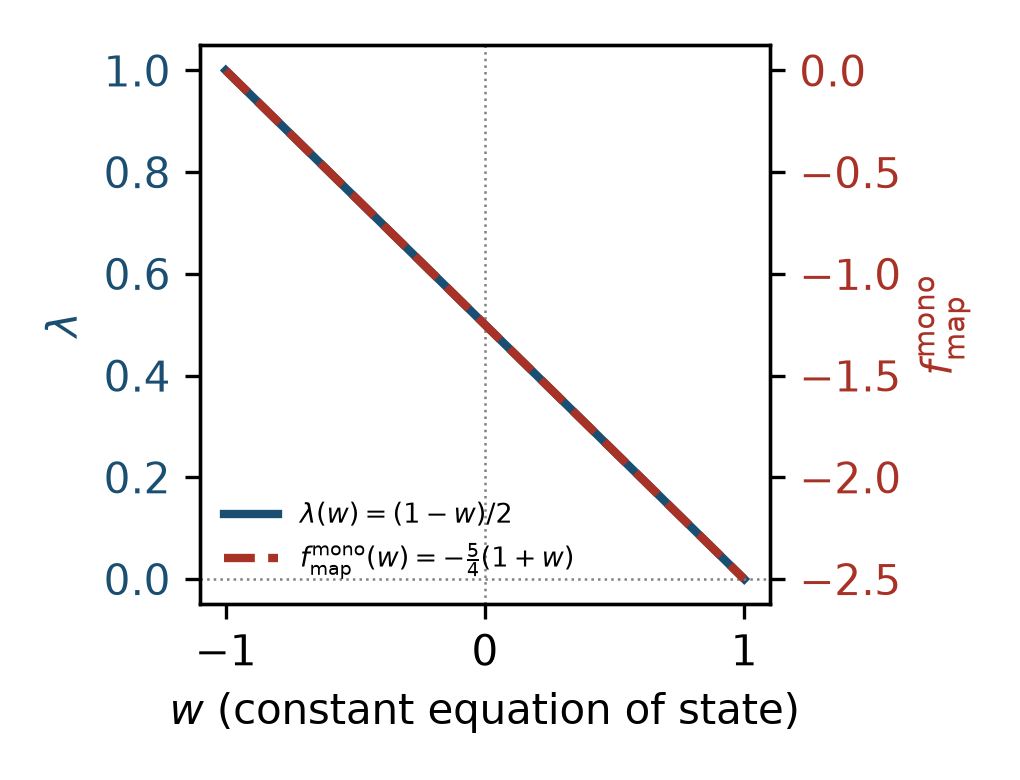
\includegraphics[width=\columnwidth]{fig_lambda_fmap.png}
\caption{The linear rescaling $\lambda(w)=(1-w)/2$ and the second-order map monopole
$f_{\rm map}^{\rm mono}(w)=-\tfrac54(1+w)$, Eq.~\eqref{eq:generalw}, for constant equation
of state $-1\le w\le1$ at $c_s=1$. Both vanish at $w=-1$ (attractor limit); $\lambda$
vanishes at $w=1$ (kination), where $\delta N_c$ loses linear response.}
\label{fig:lambda}
\end{figure}

\section{The criterion}

Equations~\eqref{eq:lambda}--\eqref{eq:fmap} give a single statement:

\emph{The isotropic separate universe ($\delta N$, with $N(\phi,\pi)$) reproduces the
squeezed bispectrum of $\zeta$ iff the $\zeta$-growth-weighted mean
$\langle\eps/c_s^2\rangle_\zeta$ vanishes. When $\langle\eps/c_s^2\rangle_\zeta=O(1)$ --
every constant-$\eps$ contraction with a growing $\zeta$ -- the two differ at $O(1)$; when
$\langle\eps/c_s^2\rangle_\zeta\ll1$ (attractor: $\dot\zeta_L=0$; USR: $\eps\ll1$
throughout the growth) they agree to $O(\langle\eps/c_s^2\rangle_\zeta)$.}

Equivalently, via the Hamiltonian constraint on comoving slices, the criterion is a
statement about the long mode's comoving density contrast: the separate universe holds
iff $\delta\rho_c/\rho\propto O(k^2/a^2H^2)\,\zeta_L$ (the gradient-expansion assumption
of Lyth, Malik \& Sasaki~\cite{Lyth2005}, following Salopek \& Bond~\cite{Salopek1990}),
and fails at $O(1)$ exactly when the long mode's Bardeen potential grows as
$\Psi_L=O((aH/k)^2)\,\zeta_L$, the textbook signature of a non-attractor
contraction~\cite{Wands1999,Finelli2002}. Two logically distinct requirements are thus
needed for $\delta N$ to work in a non-attractor phase: (i) $N(\phi,\pi)$, to capture the
growing mode as an independent initial datum~\cite{Namjoo2013}; (ii)
$\langle\eps/c_s^2\rangle_\zeta\to0$, so that the threading map is the identity. USR
satisfies (ii) approximately because $\eps\ll1$ while $\zeta$ grows -- not because the
comoving shift is small, which it is not: the shift itself is $O(1/k_L)$ in every
non-attractor, USR included, but its coefficient $\eps\dot\zeta_L$ is what controls the
$O(1)$ failure, and this coefficient is small in USR precisely when its growing-mode
initial-data problem (i) is largest. Every inflationary test cited in Sec.~I checked
(i) with (ii) automatically small; none tested a regime with $\langle\eps/c_s^2\rangle_\zeta=O(1)$.

\begin{table*}[t]
\caption{Validation of the criterion on four backgrounds (constant $\eps$, $c_s=1$
except USR). $\langle\eps\rangle_\zeta$ is the $\zeta$-growth-weighted mean of
$\eps$/$c_s^2$; $\lambda$ the linear rescaling; $f^{\rm in\text{-}in}$ the in-in monopole;
$f_{\delta N}$ the isotropic separate-universe value.}
\label{tab:validation}
\begin{ruledtabular}
\begin{tabular}{lccccc}
case & $\langle\eps\rangle_\zeta$ & $\lambda$ & $f^{\rm in\text{-}in}$ & $f_{\delta N}$ & result \\
\hline
dust, $\eps=3/2$ & $3/2$ & $1/2$ & $-35/16+\tfrac{15}{16}\mu^2$ & $-5$ & $O(1)$ fail, monopole gap $25/8$ \\
USR, $\eps\propto a^{-6}$ & $\ll1$ & $1+O(\eps)$ & $5/2$ & $5/2$ & agree to $O(\eps)$ \\
attractor slow roll & $0$ & $1$ & $\tfrac{5}{12}(1-n_s)$ & same & identity map \\
ekpyrosis, dominant mode & $0$ & $1$ & attractor-like & same & passes ($\zeta$ on constant mode) \\
\end{tabular}
\end{ruledtabular}
\end{table*}

Table~\ref{tab:validation} summarizes the four validations (script:
\texttt{separate\_uni\-verse\_failure\_criterion\_2026\_09\_04.py}, exact sympy). The dust
case ($w=0$) is the one already reported in Ref.~\cite{Golden2026Monopole}: the isotropic
separate universe gives $f_{\delta N}=-5$ for every constant $\eps\in(1,3)$, while the
in-in monopole varies with $\eps$, so the two coincide only in the limit $\eps\to0$. USR
agrees because $\eps\ll1$ throughout the growth of the long mode, exactly as the
criterion predicts, and reduces to the $N(\phi,\pi)$ result of
Ref.~\cite{Namjoo2013}. Attractor slow roll is the identity map, consistent with
Maldacena's consistency relation~\cite{Maldacena2003}. Ekpyrotic contraction ($\eps\gg3$)
passes not because the background is expanding -- it is not -- but because the physical
long mode sits on the constant-$\zeta$ solution, so $\langle\eps\rangle_\zeta=0$; this
reproduces the attractor behavior of single-field ekpyrosis found by Creminelli, Nicolis
\& Zaldarriaga~\cite{Creminelli2004}. The non-dominant, growing-$\Psi$ ekpyrotic mode would
fail by the same criterion, but never sets $\zeta_L(t_f)$ and so is not physically
realized.

\section{What is new}

Relative to Refs.~\cite{Namjoo2013,Chen2013}, this note identifies a second, independent
failure mode of $\delta N$ in non-attractors -- the threading map $\delta N_c\neq\zeta$ --
controlled by $\langle\eps/c_s^2\rangle_\zeta$ rather than by initial data, and shows it is
$O(\eps)$ in USR (hence invisible to their test) and $O(1)$ in a matter-like contraction.
Relative to Ref.~\cite{Pajer2013}, the attractor case reduces to $\Theta\equiv\eps\dot\zeta_L/(H\zeta_L)=0$
and the identity map, so the two curvature variables coincide there and the only remaining
question is observability; away from the attractor they already differ at $O(1)$ before any
observability argument, by an explicit, time-dependent, non-local map along the fluid
worldline. Relative to Ref.~\cite{Dai2015}, this note supplies the input a conformal-Fermi-coordinate
treatment of a genuine non-attractor would need: the $O(k^0)$ divergence of the long
mode's comoving shift and the resulting displacement and dilation of the local frame.
Relative to Refs.~\cite{Cai2018,Passaglia2019}, the agreement found there is explained as
the $\eps\ll1$ corner of the criterion rather than a coincidence of the USR transition.
Relative to Refs.~\cite{Bravo2018a,Bravo2018b}, the coordinate-removal argument for the
canonical single-field local $\fnl$ is $O(\eps)$-controlled in inflation; whether an
analogous physical-coordinate argument removes the $O(1)$ in-in monopole in a matter-like
contraction is a distinct, open question, not addressed here. Relative to
Refs.~\cite{Artigas2022,Jackson2023}, the mechanism and order differ: their breakdown is
localized to a finite window of scales at a slow-roll-to-USR transition and traced to a
momentum mismatch, while the criterion here applies to all super-Hubble scales at $O(k^0)$,
at constant $\eps$, with no transition required.

\section{Limits}

The second-order map, Eqs.~\eqref{eq:fmap}--\eqref{eq:generalw}, is exact for constant
$\eps$ and $c_s=1$ (the scalar-field realization of a given $w$); it is not the
second-order map for a genuine fluid with $c_s^2=w\neq1$, which needs the $c_s$-dependent
second-order ADM constraints -- an open, bounded extension. The USR second-order statement
in Sec.~III is structural (every frozen second-order kernel is proportional to $\eps$, and
vanishes as $\eps\to0$), not a re-solve with a time-dependent $\eps(t)=\eps_s(a/a_s)^{-6}$;
a full time-dependent-$\eps$ second-order calculation was not attempted. The linear
criterion, Eq.~\eqref{eq:lambda}, is exact for any single-field history and any $c_s$,
given a growing-mode initial condition.

\section*{Reproducibility Statement}
The linear criterion, second-order map, general-$w$ closed forms, and all four
validations are computed by exact sympy in the committed script
\seqsplit{research/theory\_audit/separate\_universe\_failure\_criterion\_2026\_09\_04.py}
(SHA-256 \texttt{21668ab6\ldots}), with results in the companion \texttt{.json}
(SHA-256 \texttt{4e2a49be\ldots}) and derivation in the companion note of the same base
name (\texttt{.md}); the second-order threading map is derived in
\seqsplit{threading\_map\_second\_order\_2026\_09\_04}\texttt{.\{md,py,json\}}, and the
in-in inputs in \seqsplit{fnl\_monopole\_adjudication\_2026\_09\_03.md}. Figure~\ref{fig:lambda}
is generated by \texttt{make\_fig\_lambda\_fmap.py} in this directory, transcribing the
general-$w$ closed forms with no new derivation. Manifest:
\seqsplit{reproducibility/manifests/experiments/lift2-separate-universe-failure-criterion.json}.
Local CPU, \$0, under 1~second total.

\section*{AI Usage Disclosure}
The symbolic derivations underlying this note were performed by deterministic sympy
scripts written and executed under the author's direction; every intermediate result is
printed by the committed scripts and cross-checked against the frozen inputs before use.
Claude (Anthropic) assisted with literature cross-checks, prose drafting, and LaTeX
formatting under the author's direction; all physics content, equations, and numerical
results were verified by the author against the committed script output.

\begin{thebibliography}{99}

\bibitem{Maldacena2003} J.~Maldacena, JHEP \textbf{05}, 013 (2003), arXiv:astro-ph/0210603.
\bibitem{ChenHuang2007} X.~Chen, M.~Huang, S.~Kachru, G.~Shiu, JCAP \textbf{0701}, 002 (2007), arXiv:hep-th/0605045.
\bibitem{Namjoo2013} M.~H.~Namjoo, H.~Firouzjahi, M.~Sasaki, Europhys.\ Lett.\ \textbf{101}, 39001 (2013), arXiv:1210.3692.
\bibitem{Chen2013} X.~Chen, H.~Firouzjahi, M.~H.~Namjoo, M.~Sasaki, Europhys.\ Lett.\ \textbf{102}, 59001 (2013), arXiv:1301.5699.
\bibitem{Pajer2013} E.~Pajer, F.~Schmidt, M.~Zaldarriaga, Phys.\ Rev.\ D \textbf{88}, 083502 (2013), arXiv:1305.0824.
\bibitem{Dai2015} L.~Dai, E.~Pajer, F.~Schmidt, JCAP \textbf{1511}, 043 (2015), arXiv:1504.00351.
\bibitem{Cai2018} Y.~Cai, X.~Chen, M.~H.~Namjoo, M.~Sasaki, D.-G.~Wang, Z.~Wang, JCAP \textbf{1805}, 012 (2018), arXiv:1712.09998.
\bibitem{Bravo2018a} R.~Bravo, S.~Mooij, G.~A.~Palma, B.~Pradenas, JCAP \textbf{1805}, 025 (2018), arXiv:1711.02680.
\bibitem{Bravo2018b} R.~Bravo, S.~Mooij, G.~A.~Palma, B.~Pradenas, JCAP \textbf{1805}, 024 (2018), arXiv:1711.05290.
\bibitem{Passaglia2019} S.~Passaglia, W.~Hu, H.~Motohashi, Phys.\ Rev.\ D \textbf{99}, 043536 (2019), arXiv:1812.08243.
\bibitem{Artigas2022} T.~Artigas, S.~Grain, V.~Vennin, JCAP \textbf{02}, 001 (2022), arXiv:2110.11720.
\bibitem{Jackson2023} M.~G.~Jackson \etal, arXiv:2311.03281 (2023).
\bibitem{Lyth2005} D.~H.~Lyth, K.~A.~Malik, M.~Sasaki, JCAP \textbf{0505}, 004 (2005), arXiv:astro-ph/0411220.
\bibitem{Salopek1990} D.~S.~Salopek, J.~R.~Bond, Phys.\ Rev.\ D \textbf{42}, 3936 (1990).
\bibitem{Wands1999} D.~Wands, Phys.\ Rev.\ D \textbf{60}, 023507 (1999), arXiv:gr-qc/9809062.
\bibitem{Finelli2002} F.~Finelli, R.~Brandenberger, Phys.\ Rev.\ D \textbf{65}, 103522 (2002), arXiv:hep-th/0112249.
\bibitem{Creminelli2004} P.~Creminelli, A.~Nicolis, M.~Zaldarriaga, Phys.\ Rev.\ D \textbf{71}, 063505 (2005), arXiv:hep-th/0411270.
\bibitem{Golden2026Monopole} H.~Golden, ``$f_{\rm NL}$ monopole adjudication (2026-09-03),'' \url{https://github.com/Hubify-Projects/bigbounce/blob/main/research/theory_audit/fnl_monopole_adjudication_2026_09_03.md}.
\bibitem{Golden2026Threading} H.~Golden, ``Threading map at second order (2026-09-04),'' \url{https://github.com/Hubify-Projects/bigbounce/blob/main/research/theory_audit/threading_map_second_order_2026_09_04.md}.

\end{thebibliography}

\end{document}
